\documentclass[handout, aspectratio=169]{beamer}
\mode<presentation>{}
\usepackage[utf8]{inputenc}
\usepackage{tikz}
\setbeamertemplate{theorems}[numbered]

\title{Partially ordered sets}
\author{Aryaman Maithani}
\date[01-10-2019]{1st October, 2019}
\institute[IITB]{Undergraduate\\ IIT Bombay}
\usetheme{Warsaw}
%\usecolortheme{beetle}
\newtheorem{defn}{Definition}
\newtheorem{lem}{Lemma}
\expandafter\def\expandafter\insertshorttitle\expandafter{%
  \insertshorttitle\hfill%
  \insertframenumber\,/\,\inserttotalframenumber}
\begin{document}
\begin{frame}
	\titlepage
\end{frame}
\begin{frame}{Posets}
	\begin{defn}
		A partially ordered set (or poset, for short) is a set $P$ together with a binary relation $\le$ which satisfies the following three axioms:
		\begin{enumerate}
			\item $\forall x \in P: x \le x,$
			\item $\forall x, \; y \in P: (x \le y \wedge y \le x) \implies x = y,$ and
			\item $\forall x,\;y,\;z \in P: (x \le y \wedge y \le z) \implies x \le z.$
		\end{enumerate}
	\end{defn}
	By abuse of notation, we shall often refer to $P$ as a poset, instead of $(P, \;\le)$ if there's no confusion. We may also use $\le_P$ at times when there's a possibility of confusion.\\
	We say that elements $x$ and $y$ of $P$ are comparable if either $x \le y$ or $y \le x.$ The term \emph{partially} refers to the fact that there may be elements in the poset that are not comparable.
\end{frame}
\begin{frame}{More notations}
	We also define the following three notations:
	\begin{enumerate} 
		\item $x \ge y$ iff $y \le x,$
		\item $x < y$ iff $x \le y$ and $x \neq y,$ and
		\item $x > y$ iff $y < x.$
	\end{enumerate}
	We shall also concatenate things by writing $x \le z \le y$ to mean $x \le z$ and $z \le y.$ We can extend this by concatenating more than three elements as well as using different operations such as $x \le y < z \le w.$\\~\\
	We shall also frequently use the following notation:\\
	Let $\mathbb{N}$ denote the set of positive integers.\\
	For $n \in \mathbb{N},$ define $[n] := \{k \in \mathbb{N} : k \le n\}.$\\
	That is, $[n]$ is the set of positive integers up to (and including) $n.$
\end{frame}
\begin{frame}{Examples of posets}
	Here are some examples of posets. Let $n$ be any positive integer.
	\begin{enumerate} 
		\item $[n]$ with the usual ordering of integers is a poset. Moreover, any two elements are comparable.
		\item Let $2^{[n]}$ denote all the subsets of $[n].$\\
		We can define an ordering on $2^{[n]}$ as: $A \le B$ if $A \subset B.$ As a poset, we shall denote this by $B_n.$
		\item Let $S$ denote all the positive integer divisors of $n.$\\
		Define an ordering on $S$ as: $a \le b$ if $a | b.$ As a poset, we shall denote this by $D_n.$
		\item Let $P$ denote the set of (set) partitions of $[n].$ \\
		Define an ordering on $P$ as: $\pi \le \sigma$ if every block of $\pi$ is contained in a block of $\sigma.$ As a poset, we shall denote this by $\Pi_n.$\\
		As an example, let $n = 5.$ Take $\pi = [1][234][5]$ and $\sigma = [1][2345].$ Then, we have it that $\pi \le \sigma.$
		\item In general, any collection of sets can be ordered by inclusion to form a poset.
	\end{enumerate}
\end{frame}
\begin{frame}{Isomorphism}
	Let $P$ and $Q$ be two posets.\\
	An isomorphism is a map $\varphi:P \to Q$ such that $\varphi$ is a bijection and 
	\[x \le_P y \iff \varphi(x) \le_Q \varphi(y)\text{ for every }x\text{ and }y\text{ in }P.\]\\
	Two posets $P$ and $Q$ are said to be isomorphic if there exists an isomorphism from $P$ to $Q.$ We denote this by writing $P \cong Q.$\\~\\
	What this really means is that $P$ and $Q$ are identical in terms of their structure as a poset and the elements of $P$ could simply be relabeled to give $Q.$
\end{frame}
\begin{frame}{Subposets}
	\begin{defn}[Weak subposet]
		By a weak subposet of $P,$ we mean a subset $Q$ of $P$ together with a partial ordering of $Q$ such that $x \le_Q y \implies x \le_Q y$ for all $x$ and $y$ in $Q.$
	\end{defn}
	If $Q$ is a weak subposet of $P$ and $Q = P$ as sets, then $P$ is called a \emph{refinement} of $Q.$
	\begin{defn}[Induced subposet]
		By an induced subposet of $P,$ we mean a subset $Q$ of $P$ together with a partial ordering of $Q$ such that $x \le_Q y \iff x \le_Q y$ for all $x$ and $y$ in $Q.$
	\end{defn}
	Unless otherwise mentioned, by a subposet of $P,$ we shall always mean an induced subposet.\\
	If $|P| < \infty,$ then there exist exactly $2^{|P|}$ induced subposets of $P.$
\end{frame}
\begin{frame}{Intervals}
	\begin{defn}
		A special subposet of $P$ is the (closed) interval $[x,\;y] = \{z \in P : x \le z \le y\}$ defined whenever $x \le y.$
	\end{defn}
	By definition, it should be clear that $\emptyset$ is \emph{not} an interval.\\
	Also, note that $[x,\;x] = \{x\}.$
	\begin{defn}[Locally finite poset]
		If every interval of $P$ is finite, then $P$ is called a locally finite poset.
	\end{defn}
	Examples of locally finite posets are: $B_n,\; \mathbb{N},\; \mathbb{Z}.$\\
	Examples of non-locally finite posets are: $2^\mathbb{N},\;\mathbb{R},\;\mathbb{Q}.$\\
	($2^\mathbb{N}$ denotes the power set of $\mathbb{N}$ which is a poset when ordered by inclusion.)\\
	($\mathbb{N},\;\mathbb{Z},\;\mathbb{R},\;\mathbb{Q}$ have their usual ordering.)
\end{frame}
\begin{frame}{Finite posets}
	\begin{defn}
		A poset $(P,\;\le)$ is said to be finite if $P$ is finite.
	\end{defn}
	Every finite poset is locally finite but the converse is not true as we saw earlier in the case of $\mathbb{Z}.$
\end{frame}
\begin{frame}{Convexity and covering}
	\begin{defn}[Convex subposets]
		We define a subposet $Q$ of $P$ to be convex if $y \in Q$ whenever $x < y < z$ and $x, \; z \in Q.$
	\end{defn}
	Thus, an interval is always convex.
	\begin{defn}[Cover]
		If $x,\; y\in P,$ then we say that $y$ covers $x$ if $x < y$ and $\not\exists z \in P$ such that $x < z < y.$
	\end{defn}
	The above is equivalent to saying that $x < y$ and $[x,\;y] = \{x,\;y\}.$\\
	A locally finite poset $P$ is completely determined by its cover relations.
\end{frame}
\begin{frame}{Hasse diagrams}
	The Hasse diagram of a finite poset $P$ is the graph whose vertices are the elements of $P,$ whose edges are cover relations, and such that if $x < y,$ then $y$ is drawn ``above'' $x.$ 
	\begin{figure}[h]
		\centering
		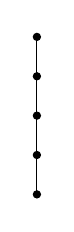
\begin{tikzpicture}
	\node (1) at (0, 0) {};
	\node (2) at (0, 0.5) {};
	\node (3) at (0, 1) {};
	\node (4) at (0, 1.5) {};
	\node (5) at (0, 2) {};
		\draw[fill=black] (1) circle (.3ex);
		\draw[fill=black] (2) circle (.3ex);
		\draw[fill=black] (3) circle (.3ex);
		\draw[fill=black] (4) circle (.3ex);
		\draw[fill=black] (5) circle (.3ex);
	\draw[shorten <= -3.5pt, shorten >= -3.5pt] (1) -- (2);
	\draw[shorten <= -3.5pt, shorten >= -3.5pt] (2) -- (3);
	\draw[shorten <= -3.5pt, shorten >= -3.5pt] (3) -- (4);
	\draw[shorten <= -3.5pt, shorten >= -3.5pt] (4) -- (5);
\end{tikzpicture}
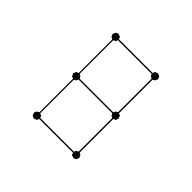
\begin{tikzpicture}
	\def \hor{ 0.5 };
	\def \ver{ 0.5 };
	\def \short{ -6 };
	\node (0) at (1*\hor,0*\ver) {};
	\node (1) at (0*\hor,1*\ver) {};
	\node (2) at (2*\hor,1*\ver) {};
	\node (3) at (1*\hor,2*\ver) {};
	\node (4) at (3*\hor,2*\ver) {};
	\node (5) at (2*\hor,3*\ver) {};
	\draw[fill=black] (0) circle (.3ex);
	\draw[fill=black] (1) circle (.3ex);
	\draw[fill=black] (2) circle (.3ex);
	\draw[fill=black] (3) circle (.3ex);
	\draw[fill=black] (4) circle (.3ex);
	\draw[fill=black] (5) circle (.3ex);
	\draw[shorten <= \short, shorten >= \short] (0) -- (1);
	\draw[shorten <= \short, shorten >= \short] (0) -- (2);
	\draw[shorten <= \short, shorten >= \short] (1) -- (3);
	\draw[shorten <= \short, shorten >= \short] (2) -- (3);
	\draw[shorten <= \short, shorten >= \short] (2) -- (4);
	\draw[shorten <= \short, shorten >= \short] (3) -- (5);
	\draw[shorten <= \short, shorten >= \short] (4) -- (5);
\end{tikzpicture}
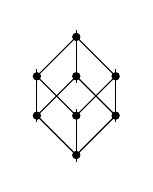
\begin{tikzpicture}
	\def \hor{ 0.5 };
	\def \ver{ 0.5 };
	\def \short{ -6 };
	\node (0) at (1*\hor,0*\ver) {};
	\node (1) at (0*\hor,1*\ver) {};
	\node (2) at (1*\hor,1*\ver) {};
	\node (3) at (2*\hor,1*\ver) {};
	\node (4) at (0*\hor,2*\ver) {};
	\node (5) at (1*\hor,2*\ver) {};
	\node (6) at (2*\hor,2*\ver) {};
	\node (7) at (1*\hor,3*\ver) {};

	\draw[fill=black] (0) circle (.3ex);
	\draw[fill=black] (1) circle (.3ex);
	\draw[fill=black] (2) circle (.3ex);
	\draw[fill=black] (3) circle (.3ex);
	\draw[fill=black] (4) circle (.3ex);
	\draw[fill=black] (5) circle (.3ex);
	\draw[fill=black] (6) circle (.3ex);
	\draw[fill=black] (7) circle (.3ex);
	\draw[shorten <= \short, shorten >= \short] (0) -- (1);
	\draw[shorten <= \short, shorten >= \short] (0) -- (2);
	\draw[shorten <= \short, shorten >= \short] (0) -- (3);
	\draw[shorten <= \short, shorten >= \short] (1) -- (4);
	\draw[shorten <= \short, shorten >= \short] (1) -- (5);
	\draw[shorten <= \short, shorten >= \short] (2) -- (4);
	\draw[shorten <= \short, shorten >= \short] (2) -- (6);
	\draw[shorten <= \short, shorten >= \short] (3) -- (5);
	\draw[shorten <= \short, shorten >= \short] (3) -- (6);
	\draw[shorten <= \short, shorten >= \short] (4) -- (7);
	\draw[shorten <= \short, shorten >= \short] (5) -- (7);
	\draw[shorten <= \short, shorten >= \short] (6) -- (7);
\end{tikzpicture}
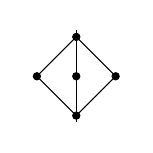
\begin{tikzpicture}
	\def \hor{ 0.5 };
	\def \ver{ 0.5 };
	\def \short{ -6 };
	\node (0) at (1*\hor,0*\ver) {};
	\node (1) at (0*\hor,1*\ver) {};
	\node (2) at (1*\hor,1*\ver) {};
	\node (3) at (2*\hor,1*\ver) {};
	\node (4) at (1*\hor,2*\ver) {};
	\draw[fill=black] (0) circle (.3ex);
	\draw[fill=black] (1) circle (.3ex);
	\draw[fill=black] (2) circle (.3ex);
	\draw[fill=black] (3) circle (.3ex);
	\draw[fill=black] (4) circle (.3ex);
	\draw[shorten <= \short, shorten >= \short] (0) -- (1);
	\draw[shorten <= \short, shorten >= \short] (0) -- (2);
	\draw[shorten <= \short, shorten >= \short] (0) -- (3);
	\draw[shorten <= \short, shorten >= \short] (1) -- (4);
	\draw[shorten <= \short, shorten >= \short] (2) -- (4);
	\draw[shorten <= \short, shorten >= \short] (3) -- (4);
\end{tikzpicture}
	\caption{Hasse Diagrams of $[5],\;D_{12},\;B_3,$ and $\Pi_3$}
	\end{figure}

	Note that given the same poset, one may make different \emph{looking} Hasse diagrams. If two posets have the same Hasse diagram, then they are clearly isomorphic.
\end{frame}
\begin{frame}{$\hat{0}$ and $\hat{1}$}
	We say that $P$ has a $\hat{0}$ if there exists an element $\hat{0} \in P$ such that $\hat{0} \le x$ for all $x \in P.$\\
	Similarly, $P$ has a $\hat{1}$ is there exists an element $\hat{1} \in P$ such that $x \le \hat{1}$ for all $x \in P.$\\
	We denote by $\hat{P}$ the poset obtained by adjoining a $\hat{0}$ and a $\hat{1}$ to $P.$ This is regardless of whether or not $P$ had a $\hat{0}$ or a $\hat{1}$ to begin with.\\
	Note that $\hat{0}$ and $\hat{1}$ \emph{have} to comparable with every element, by definition.
	\begin{figure}[h]
		\centering
		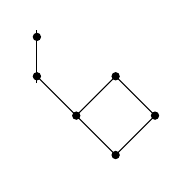
\begin{tikzpicture}
			\def \hor{ 0.5 };
			\def \ver{ 0.5 };
			\def \short{ -6 };
			\node (0) at (2*\hor,0*\ver) {};
			\node (2) at (1*\hor,1*\ver) {};
			\node (1) at (3*\hor,1*\ver) {};
			\node (4) at (0*\hor,2*\ver) {};
			\node (3) at (2*\hor,2*\ver) {};
			\node (5) at (0*\hor,3*\ver) {};
			\draw[fill=black] (0) circle (.3ex);
			\draw[fill=black] (1) circle (.3ex);
			\draw[fill=black] (2) circle (.3ex);
			\draw[fill=black] (3) circle (.3ex);
			\draw[fill=black] (4) circle (.3ex);
			\draw[fill=black] (5) circle (.3ex);
			\draw[shorten <= \short, shorten >= \short] (0) -- (1);
			\draw[shorten <= \short, shorten >= \short] (0) -- (2);
			\draw[shorten <= \short, shorten >= \short] (1) -- (3);
			\draw[shorten <= \short, shorten >= \short] (2) -- (3);
			\draw[shorten <= \short, shorten >= \short] (2) -- (4);
			\draw[shorten <= \short, shorten >= \short] (4) -- (5);
		\end{tikzpicture}
		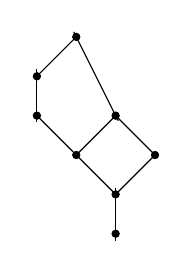
\begin{tikzpicture}
			\def \hor{ 0.5 };
			\def \ver{ 0.5 };
			\def \short{ -6 };
			\node (7) at (2*\hor,0*\ver) {};
			\node (0) at (2*\hor,1*\ver) {};
			\node (2) at (1*\hor,2*\ver) {};
			\node (1) at (3*\hor,2*\ver) {};
			\node (4) at (0*\hor,3*\ver) {};
			\node (3) at (2*\hor,3*\ver) {};
			\node (5) at (0*\hor,4*\ver) {};
			\node (6) at (1*\hor,5*\ver) {};
			\draw[fill=black] (0) circle (.3ex);
			\draw[fill=black] (1) circle (.3ex);
			\draw[fill=black] (2) circle (.3ex);
			\draw[fill=black] (3) circle (.3ex);
			\draw[fill=black] (4) circle (.3ex);
			\draw[fill=black] (5) circle (.3ex);
			\draw[fill=black] (6) circle (.3ex);
			\draw[fill=black] (7) circle (.3ex);
			\draw[shorten <= \short, shorten >= \short] (0) -- (1);
			\draw[shorten <= \short, shorten >= \short] (0) -- (2);
			\draw[shorten <= \short, shorten >= \short] (1) -- (3);
			\draw[shorten <= \short, shorten >= \short] (2) -- (3);
			\draw[shorten <= \short, shorten >= \short] (2) -- (4);
			\draw[shorten <= \short, shorten >= \short] (3) -- (6);
			\draw[shorten <= \short, shorten >= \short] (4) -- (5);
			\draw[shorten <= \short, shorten >= \short] (5) -- (6);
			\draw[shorten <= \short, shorten >= \short] (7) -- (0);
		\end{tikzpicture}
		\caption{$P$ and $\hat{P}$}
	\end{figure}
\end{frame}

\begin{frame}{Extremal elements}
	\begin{defn}
		We say that $x \in P$ is a minimal element if $y \le x \implies y = x$ for all $y \in P.$
	\end{defn}
	\begin{defn}
		We say that $x \in P$ is a maximal element if $y \ge x \implies y = x$ for all $y \in P.$
	\end{defn}
	Note that a poset may not have a minimal or a maximal element to begin with. Example - $\mathbb{N}$\\
	Even if a minimal (or maximal) element exists, it need not be unique. Example - $\{2,\;3\}$ regarded as a subposet of $D_6.$ All the elements are minimal as well as maximal.\\
	The above example also illustrates that a minimal (maximal) element need not necessarily be $\hat{0}$ $(\hat{1}).$ This sort of behaviour is precisely due to the fact that two elements may not be comparable.
\end{frame}

\begin{frame}{Chains}
	\begin{defn}
	A chain (or totally ordered set) is a poset in which any two elements are comparable. 
	\end{defn}
\begin{defn}
	A subset $C$ of $P$ is called a chain if $C$ is a chain when regarded as a subposet of $P.$
\end{defn}
\begin{defn}
	A chain $C$ of $P$ is called saturated (or unrefinable) if there does not exist $z \in P\setminus C$ such that $x < z < y$ for some $x,\;y\in C$ and $C \cup \{z\}$ is still a chain.
\end{defn}
\begin{defn}
	A chain $C$ of $P$ is called maximal if there does not exist $z \in P\setminus C$ such that $C \cup \{z\}$ is still a chain.
\end{defn}
\end{frame}

\begin{frame}{Examples}
	Consider $P = D_{30}$ and the following subsets of $P:$
	\begin{enumerate} 
		\item $C_1 = \{1,\;15,\;30\}.$ $C_1$ is a chain but not saturated as $1 < 5 < 15$ and $C_1 \cup \{5\}$ is still a chain. For similar reasons, it is not maximal either.
		\item $C_2 = \{1,\;5,\;15\}.$ $C_2$ is a chain. It is saturated as well. However, it is not maximal.
		\item $C_3 = \{1,\;5,\;15,\;30\}$ is a maximal (and saturated) chain.
		\item $C_4 = P$ is not a chain. Note that $C_4$ is an interval. Thus, intervals need not be chains.
	\end{enumerate}
	In a locally finite poset, a chain $x_0 < x_1 < \cdots < x_n$ is saturated if and only if $x_i$ covers $x_{i-1}$ for all $i \in [n].$
\end{frame}

\begin{frame}{Lengths}
	\begin{defn}
		The length of a finite chain $C$ is denoted by $l(C)$ and is defined as $l(C) := |C| - 1.$
	\end{defn}
	\begin{defn}
		The length (or rank) of a finite poset is $l(P) := \max\{l(C) : C\text{ is a chain of}P\}.$
	\end{defn}
	The length of an interval $[x,\;y]$ is denoted by $l(x,\;y).$
	\begin{defn}
		If every maximal chain of $P$ has the length $n \in \mathbb{N} \cup \{0\},$ then we say that $P$ is graded of rank $n.$
	\end{defn}
		Before proving a result about graded posets, let us see the notion of something known as a \emph{rank function.}
\end{frame}

\begin{frame}{Rank function}
	\begin{defn}
		A rank function of a poset $P$ is a function $\rho:P \to \mathbb{N}\cup\{0\}$ having the following properties:
		\begin{enumerate} 
			\item if $x$ is minimal, then $\rho(x) = 0,$ and
			\item if $y$ covers $x,$ then $\rho(y) = \rho(x) + 1.$
		\end{enumerate}
	\end{defn}
%
	Note that saying ``\emph{a} rank function'' instead of ``\emph{the} rank function'' has a subtlety.\\
	Given an arbitrary poset $P,$ it is \textbf{not} necessary that is has a rank function. For example, $\mathbb{Z}$ has no rank function. Also, given a poset $P,$ it \emph{may} have more than one rank functions as well. As an example, the set of nonnegative real numbers has infinitely many rank functions!\\
	Even a finite poset need not have a rank function. Example- $\{2,\;6,\;15,\;30\}$ regarded as a subposet of $D_{30}.$
\end{frame}
\begin{frame}{Some rank theorems}
	\begin{theorem}\label{thm:uni}
		Every graded poset possesses a unique rank function.
	\end{theorem}
	It is important to observe that even if the poset is not finite, it could still be graded. For example, $(\mathbb{N}, \; =)$ is graded of rank $0.$\\
	Before we prove Theorem \ref{thm:uni}, let us see another theorem.\\
	\begin{theorem}\label{thm:intlen}
		If $x \le y,$ then $l(x,\;y) = \rho(y) - \rho(x).$
	\end{theorem}
	Given an element $x$ of a graded poset, the existence and uniqueness of a rank function lets us talk about the rank of $x.$ We define rank of $x$ to be $\rho(x),$ where $\rho$ is the unique rank function.
\end{frame}
\begin{frame}{A lemma}
	\begin{lem}\label{lem:unichain}
		Every finite chain possesses a unique rank function.
	\end{lem}
	\begin{proof}
		Assume $C = \{x_0,\;x_1,\;\ldots,\;x_n\}$ is a finite chain of length $n$ such that $x_0 < x_1 < \cdots x_n.$ Then, $x_0$ is a minimal element of $C,$ and for all $i \in [n],$ we have it that $x_i$ covers $x_{i-1}.$ Define $\rho:C \to \mathbb{N}\cup\{0\}$ by defining $\rho(x_i) = i.$ Then, $\rho$ satisfies the properties of a rank function. This shows the existence of a rank function.\\~\\
		Suppose $\rho'$ were another rank function of $C$ different from $\rho.$ It is forced that $\rho'(x_0) = 0.$ Thus, for some $i \in [n],$ $\rho(x_i) \neq \rho'(x_i).$\\
		If $\rho(x_i) < \rho(x_i)',$ then $\rho'(x_0) = \rho'(x_1) - 1 = \cdots = \rho'(x_i) - i > i - i = 0,$ a contradiction.\\
		Similarly, if $\rho(x_i) < \rho(x_i)',$ we get that $\rho'(x_0) < 0,$ a contradiction.
	\end{proof}
\end{frame}
\begin{frame}{Proof of Theorem \ref{thm:uni}}
	Assume $P$ is a graded poset of rank $n.$ Let $C = \{x_0,\;x_1,\;\ldots,\;x_n\}$ be an arbitrary maximal chan of $P$ such that $x_0 < x_1 < \cdots < x_n.$ By Lemma \ref{lem:unichain}, there exists a unique rank function $\rho_C$ for $C.$\\
	Let $C' = \{x_0',\;x_1',\;\ldots,\;x_n'\}$ be any other maximal chain such that $x_0' < x_1' < \cdots < x_n'$ and $C \cap C' \neq \emptyset.$ Let $\rho_{C'}$ be the unique rank function for $C'$ and suppose that for some $x \in C \cap C',$ $\rho_C(x) \neq \rho_{C'}(x).$\\
	Then, there exist $i,\;j \in [n]\cup\{0\}$ such that $i \neq j$ and $x = x_i = x_j'.$ Without loss of generality, we can assume that $j > i.$\\
	Then, $\{x_0',\; x_1,\;\ldots,\;x_j' = x_i,\;\ldots,\;x_n\}$ is a chain of length $j + n - i > n,$ which contradicts the assumption of the rank of $P.$\\
	Thus, we have shown that given any chains, their rank functions agree on the common values, if any.\\
	Since $P = \bigcup\{C \subset P : C \text{ is a maximal chain of }P\},$ we can define $\rho(x) = \rho_C(x)$ where $C$ is any maximal chain containing $x.$ This map is well defined by our above exercise and its uniqueness follows from the uniqueness of each $\rho_C.$ \hfill $\qed$
\end{frame}
\begin{frame}{Proof of Theorem \ref{thm:intlen}}
	Assume $P$ is a graded poset of of rank $n$ with rank function $\rho.$ Given $x \le y$ in P, let $C = \{x_0,\;x_1,\;\ldots,\;x_n\}$ be a maximal chain of $P$ containing $x$ and $y$ such that $x_0 < x_1 < \cdots < x_n.$\\
	Then, for some $i,\;j\in [n]\cup\{0\}$ such that $i < j,$ we have that $x_i = x$ and $x_j = y.$ This forces $l(x,\;y) = j - i.$ Else wise, we would get that $l(C) \neq n.$\\
	But by Theorem \ref{thm:uni}, we know that $\rho(y) = j$ and $\rho(x) = i.$ \hfill $\qed$
\end{frame}
\begin{frame}{More on graded posets}
	\begin{defn}
		If $P$ is a finite graded poset of rank $n$ such that for each $i \in [n] \cup\{0\},$ $p_i$ is the number of elements of $P$ of rank $i,$ then the rank-generating function of $P$ is the polynomial
		\[F(p,\;x) := \sum_{i=0}^{n}p_ix^i.\]
	\end{defn}
	Most of the posets we saw so far were graded. Examples - $[n],\;B_n,\;D_n,$ and $\Pi_n.$

\end{frame}
	
\begin{frame}{Some examples}
	
	\begin{tabular}{|c|c|c|c|}
	\hline 
	Poset $P$ & Rank of $x \in P$ & Rank of $P$ & $F(P,\;x)$\\
	\hline
	$[n]$ & $x - 1$ & $n - 1$ & $\displaystyle\sum_{i=0}^{n-1}x^i$\\
	$B_n$ & $|x|$ & $n$ & $\displaystyle\sum_{i=0}^{n}\binom{n}{i}x^i$\\
	& & & \\
	$D_n$ & \begin{tabular}{c}number of prime \\ divisors of $x$ \end{tabular} & \begin{tabular}{c}number of prime\\ divisors of $n$ \end{tabular} & \begin{tabular}{c} $F(B_n,\;x),$\\ if $n$ is square free\end{tabular}\\
	& & & \\
	$\Pi_n$ & $n - |x|$ & $n - 1$ & $\displaystyle\sum_{i=0}^{n-1}S(n, n-i)x^i$\\
	\hline
	\end{tabular}

	Where $S(n,\;k) = \dfrac{1}{k!}\displaystyle\sum_{i=0}^{k}(-1)^{k-i}\binom{k}{i}i^n$ is a Stirling number of the second kind.
\end{frame}
\begin{frame}{Antichains and ideals}
	\begin{defn}[Antichain]
		An antichain is a subset $A$ of a poset $P$ such that any two distinct elements of $A$ are not comparable.
	\end{defn}
	\begin{defn}[Order ideal]
		An order ideal of a poset $P$ is a subset $I$ of $P$ such that if $x \in I$ and $y \le x,$ then $y \in I.$
	\end{defn}
	When $|P| < \infty,$ there is a one-to-one correspondence between antichains $A$ of $P$ and order ideals $I$ of $P.$\\
	Given an antichain $A,$ one can construct an order ideal $I$ as follows: $I = \{x \in P : x \le y \text{ for some }y \in A\}.$\\
	Similarly, given an order ideal $I,$ one can construct an antichain $A$ as follows: $A = \{x \in I : x \text{ is a maximal element of }I\}.$ \hfill $(*)$
\end{frame}
\begin{frame}{More on order ideals}
	The set of all order ideals of $P,$ ordered by inclusion, forms a poset which is denoted by $J(P).$ If $I$ and $A$ are related as in $(*),$ then we say that $A$ \emph{generates} $I.$ If $A = \{x_1, x_2, \ldots, x_k\},$ then we write $I = \langle x_1, x_2, \ldots, x_k\rangle$ for the order ideal generated by $A.$\\~\\
	The order ideal $\langle x\rangle$ is the principal order ideal generated by $x,$ denote $\Lambda_x.$
\end{frame}
\begin{frame}{New posets from old}
	We shall now see some operations on posets that let us create new posets.
\end{frame}
\begin{frame}{Direct sum}
	\begin{defn}[Direct sum]
		If $(P,\; \le_P)$ and $(Q,\;\le_Q)$ are posets on disjoint sets, then the direct sum of $P$ and $Q$ is the poset $P + Q$ defined on $P\cup Q$ such that $x \le y$ in $P+Q$ if either
		\begin{enumerate} 
			\item $x,\;y\in P$ and $x \le_P y,$ or
			\item $x,\;y\in Q$ and $x \le_Q y.$
		\end{enumerate}
	\end{defn}
	A poset that is not (isomorphic to) a disjoint union of two nonempty posets is said to be connected.\\
	Examples - 
	\begin{enumerate} 
		\item $[5]$ is connected.
		\item The subposet $\{4,\;6\}$ of $D_{12}$ is not connected. $\{4,\;6\} \cong \{4\} + \{6\}.$
	\end{enumerate}
	The disjoint union of $P$ with itself $n$ times is denoted by $nP.$\\
	An $n-$element antichain is isomorphic to $n[1].$
\end{frame}
\begin{frame}{Ordinal sum}
	\begin{defn}[Ordinal sum]
		If $P$ and $Q$ are disjoint sets as above, then the ordinal sum of the posets $P$ and $Q,$ denoted by $P\oplus Q$ is the poset defined on $P\cup Q$ such that $x \le y$ in $P\oplus Q$ if
		\begin{enumerate} 
			\item $x,\;y\in P$ and $x \le_P y,$ or
			\item $x,\;y\in Q$ and $x \le_Q y,$ or
			\item $x\in P$ and $y\in Q.$
		\end{enumerate}
	\end{defn}
	Hence, an $n-$element chain is isomorphic to $\underbrace{[1]\oplus[1]\oplus\cdots\oplus[1]}_{n \text{ times}}.$\\
	Posets that can be built up using disjoint union and ordinal sums from the poset $[1]$ are called series-parallel posets.\\
	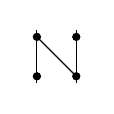
\begin{tikzpicture}
		\def \hor{ 0.5 };
		\def \ver{ 0.5 };
		\def \short{ -6 };
		\node (0) at (0*\hor,0*\ver) {};
		\node (1) at (1*\hor,0*\ver) {};
		\node (2) at (0*\hor,1*\ver) {};
		\node (3) at (1*\hor,1*\ver) {};
		\draw[fill=black] (0) circle (.3ex);
		\draw[fill=black] (1) circle (.3ex);
		\draw[fill=black] (2) circle (.3ex);
		\draw[fill=black] (3) circle (.3ex);
		\draw[shorten <= \short, shorten >= \short] (0) -- (2);
		\draw[shorten <= \short, shorten >= \short] (1) -- (2);
		\draw[shorten <= \short, shorten >= \short] (1) -- (3);
	\end{tikzpicture}
	This is the only poset (up to isomorphism) with four elements that is not series-parallel.
\end{frame}
\begin{frame}{Direct Product}
	\begin{defn}
		If $(P, \le_P)$ and $(Q, \le_Q)$ are posets, then the direct product of $P$ and $Q$ is the poset $P \times Q = (P \times Q, \le_{P \times Q})$ such that $x \le_{P \times Q} y$ if $x \le_P x'$ and $y \le_Q y'.$\\
	\end{defn}
	The direct product of $P$ with itself $n$ times is denoted by $P^n.$\\
	To draw the Hasse diagram of $P \times Q,$ (when $P$ and $Q$ are finite) we do the following:
	\begin{enumerate} 
		\item Draw the Hasse diagram of $P.$
		\item Replace every element $x \in P$ by a copy $Q_x$ of $Q.$
		\item Connect corresponding elements of $Q_x$ and $Q_y$ if $x$ and $y$ are connected in the Hasse diagram of $P.$
	\end{enumerate}
	It is clear from the definition that $P\times Q \cong Q \times P.$ However, using the above procedure, the Hasse diagrams may \emph{look} completely different.
\end{frame}
\begin{frame}{A theorem on rank generating functions}
	\begin{theorem}
		If $P$ and $Q$ are graded with rank-generating functions $F(P, x)$ and $F(Q, x),$ then $P \times Q$ is graded and $F(P\times Q, x) = F(P, x)F(Q, x).$
	\end{theorem}
	Before proving this theorem, we shall first prove the following lemma:
	\begin{lem}
		If both $P$ and $Q$ have finite lengths, then $l(P\times Q) = l(P) + l(Q).$
	\end{lem}
\end{frame}
\begin{frame}{Proof of the lemma}
	
	\begin{proof}
		Assume $P$ has length $m$ and $Q$ has length $n.$ Given any arbitrary chains $C = \{(x_0, y_0), \ldots, (x_l, y_l)\}$ of $P \times Q$ such that $(x_0, y_0) <_{P \times Q} \cdots <_{P \times Q} (x_l, y_l),$ it follows that $X = \{x_0, \ldots, x_l\}$ is a chain of $P$ and $Y = \{y_0, y_1, \ldots, y_l\}$ is a chain of $Q.$ Note that for each $i \in [l],$ $(x_{i-1}, y_{i-1}) <_{P \times Q} (x_i, y_i)$ implies that $x_{i-1} <_P x_i$ or $y_{i - 1} <_Q y_i.$ Since $l(P) = m,$ we get that $x_{i-1} < x_i$ is true for at most $m$ many elements in $[l]$ and similarly $y_{i-1} < y_i$ is true for at most $n$ many elements. Thus, we get that $l \le m + n.$\\
		Now, we actually produce a chain of length $m + n.$ As $P$ has length $m,$ there exists a chain $C_1 = \{x_0, x_1,\ldots, x_m\}$ of $P$ such that $x_0 <_P x_1 <_P \cdots <_P x_m.$ Similarly, there exists a chain $C_2 = \{y_0, y_1, \ldots y_m\}$ of $Q$ such that $y_0 <_Q y_1 <_Q \cdots <_Q y_m.$ \\
		Then, $\mathcal{C} = \{(x_0, y_0), (x_0, y_1), \ldots (x_0, y_n), (x_1, y_n), \ldots (x_m, y_n)\}$ is a chain of $P\times Q$ of length $m + n.$
	\end{proof}
\end{frame}
\begin{frame}{Proof of the theorem}
	Assume that $P$ and $Q$ are graded of rank $m$ and $n,$ respectively. By the previous lemma, $P \times Q$ has rank $m + n.$ Now we show that $P \times Q$ is indeed graded.\\
	Let $C = \{(x_0, y_0), (x_1, y_1), \ldots, (x_l, y_l)\}$ be an arbitrary maximal chain of $P \times Q$ such that $(x_0, y_0) <_{P \times Q} \cdots <_{P \times Q} (x_l, y_l).$ If $l < m + n,$ then there exists $i \in [l]$ such that $x_{i-1} <_P x_i$ and $y_{i-1} <_Q y_i.$ (Use an argument similar to that used in the proof of the previous lemma.)\\
	But this implies that $C \cup \{(x_{i-1}, y_i)\}$ is a chain, contradicting the maximality of $C.$ Thus, $l(C) = m + n.$ As $C$ was arbitrary, $P\times Q$ is graded of rank $m + n.$\\~\\
	Now, we shall show the relation of rank-generating functions that was stated before.
\end{frame}
\begin{frame}{Proof of the theorem}
	Assume that the rank generating functions of $P$ and $Q$ are $\sum_{i=0}^{m}p_ix^i$ and $\sum_{i=0}^{n}q_ix^i,$ respectively.\\
	Let $x \in P$ have rank $k$ and $y \in Q$ have rank $l.$ We show that $(x, y)$ has rank $k + l.$\\
	To see this, consider maximal chains $X = \{x_0, x_1,\ldots, x_m\}$ and $Y = \{y_0, y_1, \ldots, y_n\}$ of $P$ and $Q,$ respectively such that $x \in X$ and $y \in Y$ and $x_0 <_P x_1 <_P \cdots <_P x_m$ and $y_0 <_Q y_1 <_Q < \cdots y_n.$ By Theorem \ref{thm:uni}, we have it that $x = x_k$ and $y = y_l.$ The chain 
	\[C = \{(x_0, y_0), \ldots, (x_k, y_0), \ldots, (x_k, y_l), \ldots, (x_k, y_n), \ldots, (x_m, y_n)\}\]
	of $P \times Q$ such that
	\[\{(x_0, y_0) <_{P \times Q} (x_k, y_0) <_{P \times Q} (x_k, y_l) <_{P \times Q} (x_k, y_n), <_{P \times Q} (x_m, y_n)\}\]
	in $P \times Q$ has length $m + n$ and so it is maximal. It follows again, by Theorem \ref{thm:uni} that $(x, y)$ has rank $k + l.$ Thus, the number of elements of $P \times Q$ of rank $j$ is $\displaystyle\sum_{i=0}^{j}p_iq_{j-i},$ which is the coefficient of $x^j$ in $F(P, x)F(Q, x).$ \hfill $\qed$
\end{frame}
\begin{frame}{Ordinal product}
	\begin{defn}{Ordinal product}
		If $(P, \le_P)$ and $(Q, \le_Q)$ are posets, then the direct product of $P$ and $Q$ is the poset $P \otimes Q = (P \times Q, \le_{P \otimes Q})$ such that $x \le_{P \otimes Q} y$ if
		\begin{enumerate} 
			\item $x = x'$ and $y \le y',$ or
			\item $x < x'.$
		\end{enumerate}
	\end{defn}
	We state the following theorem without proof:
	\begin{theorem}
		If $P$ and $Q$ are graded and $Q$ has rank $r,$ then
		\[F(P \otimes Q, x) = F(p, x^{r+1})F(Q, x).\]
	\end{theorem}
	In general, $P \otimes Q$ and $Q \otimes P$ don't have the same rank-generating function. Thus, they are not isomorphic.
\end{frame}
\begin{frame}{Dual of a poset}
	\begin{defn}[Dual poset]
		Let $P$ be a poset. We denote by $P^*$ the poset defined on the same set as that of $P$ such that $x \le_{P^*} y \iff y \le_P x.$
	\end{defn}
	If $P$ and $P^*$ are isomorphic, then $P$ is said to be self-dual.\\
	There are eight posets (up to isomorphism) with $4$ elements that are self-dual.
\end{frame}
\end{document}